\section{Initial conditions}
The shape of a bubble is determined by the interaction of two forces: Gravity and surface tension.

Surface tension is an interfacial property of liquid that shows the elastic tendency, which is created by the attractive forces of the surface molecules



\subsection{Governing Equations}
Given the small size of the bubbles we are interested in, we can make the assumption that the cavity is initially motionless. Experiments have shown that, even in the absence of surfactants, a bubble can stay at the free surface in a quasi static equilibrium for a few seconds \cite{blanchard1988film}.
We need to determine the initial shape of a bubble floating at a gas-liquid interface before it's film ruptures. This derivation is based on the work done in \cite{toba1959drop}.

We are considering the case where the fluid is stationary, i.e. $\bf{u} = \bf{0}$, meaning on the boundaries we only need to consider the Young-Laplace equation:
\begin{align}
    \Delta p=-\gamma \nabla \cdot \hat n.
\end{align}

\begin{figure}
    \centering
    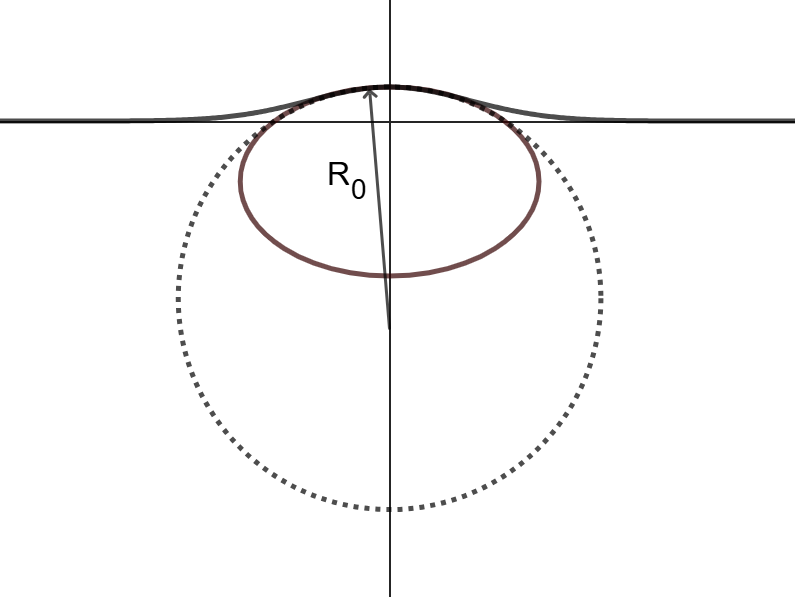
\includegraphics[width=0.7\linewidth]{WriteUp/images/bubble at surface.png}
    \caption{A bubble floating at a surface. Segment (A) in green is the Segment of the bubble which is submerged in the liquid. Segment (B) in purple is the spherical cap of the bubble, where the sphere has radius $R_0$. Segment (C) in red is the meniscus of the bubble. All three segments meet at a point.}
    \label{fig:2}
\end{figure}

We can divide the surface of a bubble into three regions: (A) the submerged segment of the interface, (B) the thin film over the top of the bubble separating the two gas regions, (C) the regions of the interface trailing away from the border of the thin film. We neglect the thickness of the film meaning we can ignore the weight of the film. Adding that the difference between the gas pressures inside and out of the bubble is uniform, the thin film can be treated as a spherical surface of radius $R_0$. The force balance equations at any point on these surfaces are,
\begin{align}\label{A_untransformed}
    (\rho-\rho')gz = \gamma \left( \frac{1}{R_1}+\frac{1}{R_2}-\frac{4}{R_0} \right)
\end{align}
for region (A),
\begin{align}\label{B_untransformed}
    p=p_0 + \frac{4\gamma}{R_0}
\end{align}
for region (B),
\begin{align}\label{C_untransformed}
    (\rho-\rho')gz = \gamma \left(\frac{1}{R_1}+\frac{1}{R_2} \right)
\end{align}
for region (C) where $\gamma$ represents surface tension of the liquid, $g$ is acceleration due to gravity, $\rho$ and $\rho'$ are the densities of the liquid and gas respectively, $p$ and $p_0$ are the gas pressure inside and outside the bubble respectively, $g$ is acceleration due to gravity and $z$ is the height above the still gas liquid interface in the far field. $R_1$ and $R_2$ are the principle radii of curvature of the surface at a point. In order to calculate what $R_1$ and $R_2$ are we need to use some differential geometry. We assume the bubble can be described by a surfaces of revolution.
Let $\Gamma$ be a curve that lies in the plane $(x,z)$ and let its equation have the equation $z=f(x)$. We then denote $\Phi$ as the surface defined by a rotation of $\Gamma$ around the $z$-axis or axis of rotation. This surface can then be written in the form:
\begin{align}
    z=f(\sqrt{x^2+y^2})=f(r), && r=\sqrt{x^2+y^2}.
\end{align}

Then using the formulas derived in \cite{toponogov2006differential} we get
\begin{align}
    E&=1+(\frac{x}{r}f')^2,&G&=1+(\frac{y}{r}f')^2, &F&=\frac{xy}{r^2}(f')^2, &EG-F^2=&1+(f')^2,
\end{align}
for the coefficients of the first fundamental form given by
\begin{align}
    I( \vec{ \boldsymbol\lambda}) = E(\lambda_1)^2 +2F\lambda_1 \lambda_2 + G(\lambda_2)^2,
\end{align}
where $\lambda$ is some tangent vector. We can exploit the fact that since our surface is radially symmetric, we only need to find these geometric characteristics on some meridian of the surface, say y=0:
\begin{align}
    E&=1+(f')^2,& G&=1, &F&=0.
\end{align}
Again using the formulas in \cite{toponogov2006differential}, we obtain
\begin{align}
    L&=\frac{f''}{\sqrt{1+(f')^2}},&M&=0,&  N&=\frac{f'}{x\sqrt{1+(f')^2}},
\end{align}
for the coefficients of the second fundamental form given by
\begin{align}
    II( \vec{ \boldsymbol\lambda},\vec{ \boldsymbol\mu}) = L\lambda_1 \mu_1 +M(\lambda_1\mu_2 + \lambda_2 \mu_1)  + N\lambda_2 \mu_2.
\end{align}
We then obtain the principle curvatures $\kappa_1$ and $\kappa_2$ satisfy:
\begin{align}
    (EG-F^2)\kappa^2 - (EN+GL -2MF)\kappa +LN-M^2 = 0.
\end{align}
Substituting in our coefficients for the first and second fundamental forms, solving for $\kappa$ and noting radius of curvature is one over the curvature we obtain:
\begin{align}
    \frac{1}{R_1} =\kappa_1= \frac{L}{E}=\frac{f''}{(1+(f')^2)^{\frac{3}{2}}}, && \frac{1}{R_2} = \kappa_2 = \frac{N}{G} = \frac{f'}{x \sqrt{1+(f')^2}}.
\end{align}
Notice that $R_1$ is exactly the radius of curvature of the meridian curve $\Gamma$
We now introduce the variable $\phi$ defined to be the angle at which the tangent to $\Gamma$ makes with the x-axis. 
\begin{figure}
    \centering
    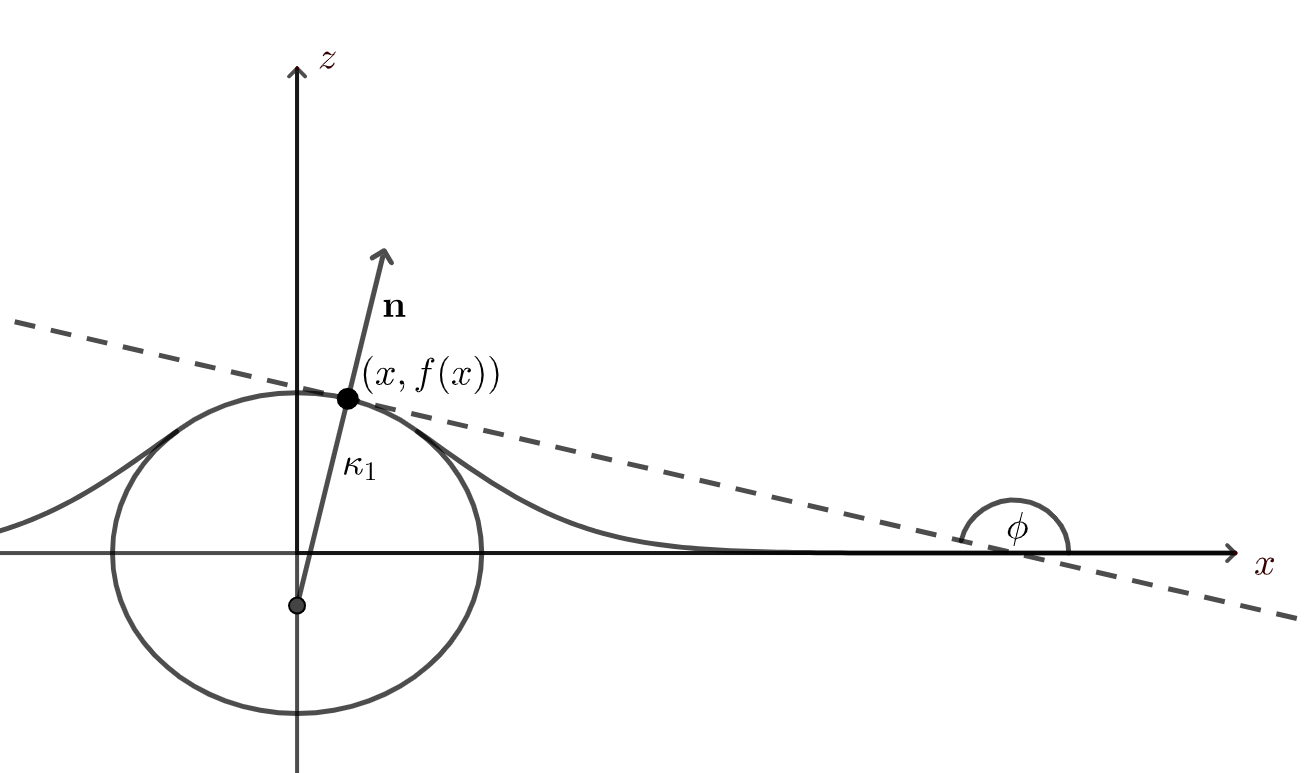
\includegraphics[width=0.75\linewidth]{WriteUp/images/tangent to bubble extra.png}
    \caption{A bubble floating at a surface with a tangent line at a point. This tangent intersects the $x$-axis with angle $\phi$}
    \label{fig:3}
\end{figure}
We can calculate $\phi$ using simple trigonometry to be $\phi=\arctan(f'(x))$. We then consider:
\begin{align}
    f'(x)=\tan \phi &= \frac{\sin\phi}{\cos\phi} 
    =\sin\phi\sec\phi 
    =\sin\phi \sqrt{1+\tan^2\phi}\\
    \frac{f'(x)}{\sqrt{1+f'(x)^2}}&=\sin\phi\\
    \frac{d}{dx} \frac{f'(x)}{\sqrt{1+f'(x)^2}}&=\frac{d}{dx}\sin\phi \\
    \frac{f''(x)}{(1+f'(x)^2)^{\frac{3}{2}}}&=\frac{d(\sin\phi)}{dx} \\
    \frac{1}{R_1}&=\frac{d(\sin\phi)}{dx}
\end{align}
Allowing us to obtain $R_1$ in terms of $\phi$. reparametrising the curve in terms of $z$, i.e. considering the curve given by $(g(z),z)$ where $g(z)=f^{-1}(z)$, we can find another expression for $R_1$. using the facts,
\begin{align}
    f'(x)=\frac{1}{g'(f(x))}, && f''(x) = \frac{-g''(f(x))}{g'(f(x))^3}
\end{align}
We can write the curvature in terms of $z$:
\begin{align}
    \frac{f''(x)}{(1+f'(x)^2)^{\frac{3}{2}}}=\frac{-\frac{g''(f(x))}{g'(f(x))^3}}{(1+\frac{1}{g'(f(x))})} = \frac{-g''(f(x))}{(g'(f(x))^2+1)^{\frac{3}{2}}} = \frac{-g''(z)}{(g'(z)+1)^{\frac{3}{2}}}
\end{align}
Now we can consider,
\begin{align}
    f'(x)=\frac{1}{g'(f(x))}=\tan \phi &= \frac{\sin\phi}{\cos\phi} \\
    g'(z)&=\cos\phi\csc\phi
    =\sin\phi \sqrt{1+\cot^2\phi}\\
    \frac{g'(z)}{\sqrt{1+g'(z)^2}}&=\cos\phi\\
    \frac{d}{dz} \frac{f'(z)}{\sqrt{1+f'(z)^2}}&=\frac{d}{dz}\cos\phi \\
    \frac{g''(z)}{(1+g'(z)^2)^{\frac{3}{2}}}&=\frac{d(\cos\phi)}{dx} \\
    \frac{1}{R_1}&=-\frac{d(\cos\phi)}{dz}
\end{align}
We can also write $R_2$ in terms of $\phi$ by considering the normal to the curve at a point $(x,f(x))$. An equation for this normal is given by
\begin{align}
    (\bar{x}-x) + f'(x)(\bar{z}-f(x))=0
\end{align}
where $(\bar{x},\bar{z})$ are the coordinates of points on the straight line. We can the find the intersection of this line with the $z$-axis, $(0,\frac{x+ff'}{f'})$.
Finding the distance $R$ between this point and $(x,f)$ gives
\begin{align}
    R=\sqrt{x^2+(\frac{x+ff'}{f'}-f)^2}=\frac{x\sqrt{1+(f')^2}}{|f'|}=R_2.
\end{align}
We can then use trigonometry to calculate $R$ in terms of $\phi$:
\begin{align}
    R=\frac{x}{\cos(\frac{\pi}{2}-\phi)}=\frac{x}{\sin(\phi)}.
\end{align}
Combining these all together we obtain
\begin{align}
    \frac{1}{R_1}&=\frac{d(\sin(\phi))}{dx},\\
    \frac{1}{R_2}&=\frac{\sin(\phi)}{x},\\
    \frac{dz}{dx} &= \tan(\phi).
\end{align}
\begin{figure}
    \centering
    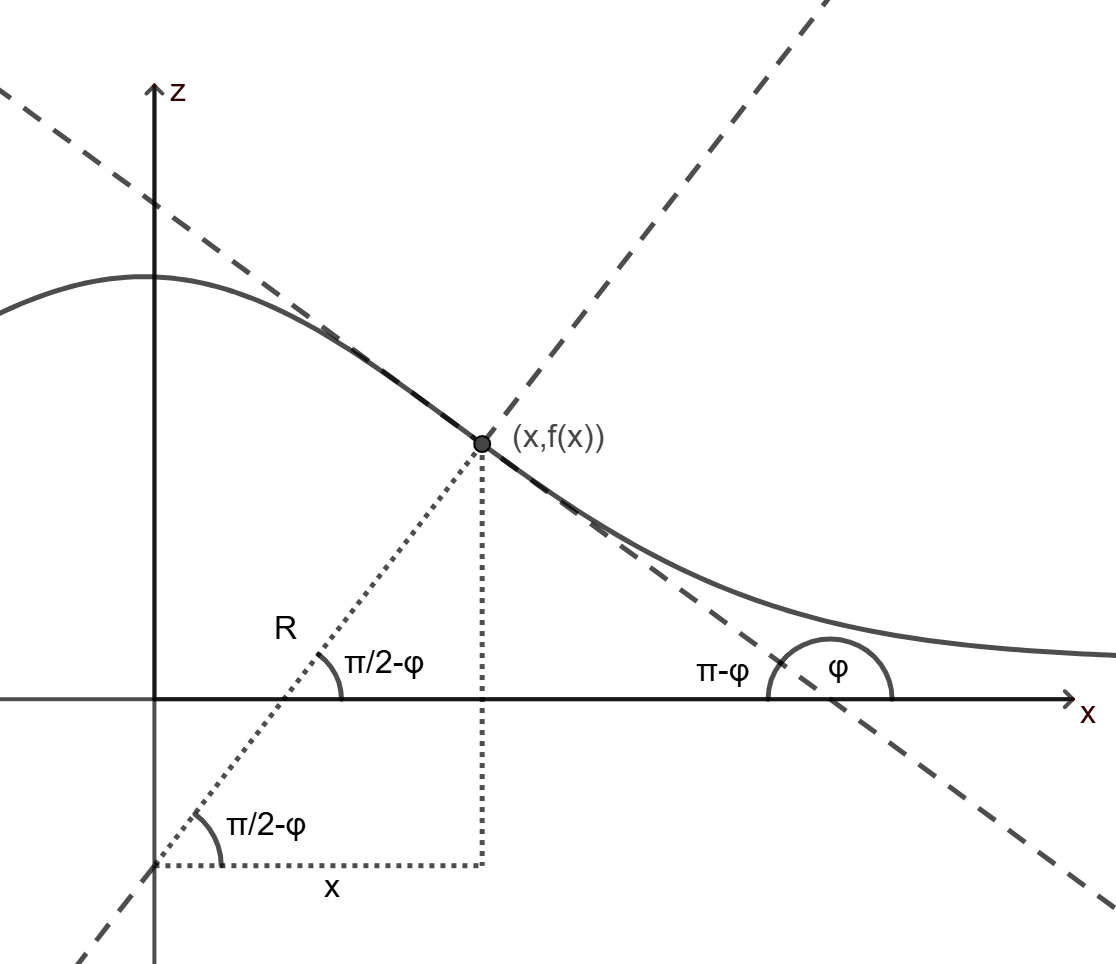
\includegraphics[width=0.75\linewidth]{WriteUp/images/angles and trig.png}
    \caption{A bubble floating at a surface. Both a tangent line and a line normal to the curve are shown at a point. The distance along the normal between the point and the $z$-axis is given by $R$}
    \label{fig:4}
\end{figure}
We now introduce a capillary constant $a^2$ having dimension of square length and defined by the equation
\begin{align}
    \frac{(\rho-\rho')g}{\gamma} = \frac{2}{a^2}
\end{align}
transform $x$, $z$, $R_0$, etc. to dimensionless quantities $\bar{x}$, $\bar{z}$, $\bar{R_0}$, etc. by
\begin{align}
    x=a\bar{x}, && z=a\bar{z}, && R_0=a\bar{R}_0, && \text{etc.}
\end{align}
We then consider two new transformed coordinates:
\begin{align}
    \bar{z}_1 = \bar{z}+\bar{h}, && \bar{z}_2=\bar{z}+\bar{l}
\end{align}
where $\bar{h}$ and $\bar{l}$ are chosen such that $\bar{z}_1$ has its origin at the deepest point of the bubble for segment (A) and $\bar{z}_2$ has its origin at the centre of the sphere for segment (B). For segment (A), instead of \ref{A_untransformed}, we obtain
\begin{align}\label{less than}
    \frac{d\bar{z}_1}{d\bar{x}} &= \tan \phi &
    \frac{d(\sin\phi)}{d\bar{x}} &= 2\bar{z}_1 - \frac{\sin\phi}{\bar{x}} + \theta
\end{align}
or,
\begin{align}\label{greater than}
    \frac{d\bar{x}}{d\bar{z}_1} &= \cot \phi & 
    \frac{d(\cos\phi)}{d\bar{z}_1} &= -2\bar{z}_1 + \frac{\sin\phi}{\bar{x}} - \theta
\end{align}
where,
\begin{align}
    \theta = \frac{4}{\bar{R}_0} - 2\bar{h}
\end{align}
and the equations \ref{less than} and \ref{greater than} are used for $\tan\phi <1$ and $\tan\phi >1$ respectively. Similarly for portion (C), equation \ref{C_untransformed} becomes,
\begin{align}\label{C_transformed}
    \frac{d\bar{z}}{d\bar{x}} &= \tan \phi &
    \frac{d(\sin\phi)}{d\bar{x}} &= 2\bar{z} - \frac{\sin\phi}{\bar{x}}
\end{align}
We can notice that equation \ref{less than} and \ref{greater than} are essentially the same of equation \ref{C_transformed} except for the additional $\theta$ term. Finally equation \ref{B_untransformed} for segment (B) becomes
\begin{align}\label{Eq_B}
    \bar{z}_2 = \sqrt{ \bar{R}_0^2+\bar{x}^2}
\end{align}
We are now ready to start solving for the initial condition.

\subsection{Solving for Segment (A)}

We have derived the governing equations for each of the three segments of the bubble and now can start to solve them. We already have an explicit expression for segment (B), although finding analytic solutions to \ref{less than}, \ref{greater than} and \ref{C_transformed} is too difficult. Instead we can find numerical solutions using a Runge-Kutta method.

First we consider the equations \ref{less than} and \ref{greater than}. We use the initial conditions $\bar{x}=\bar{z}_1=0$ at $\theta=0$ as we assume that at the bottom of the bubble is flat, i.e.
\begin{align}
    \frac{d\bar{z}_1}{d\bar{x}}&=0&
    \Leftrightarrow \:\:\:\:\:\theta&=0.
\end{align}
The relations
\begin{align}
    \frac{1}{\bar{R}_1}=\frac{\sin\phi}{\bar{x}}=\frac{1}{\bar{R}_2}=\frac{d(\sin\phi)}{d\bar{x}}=\frac{\theta}{2}
\end{align}
were also used as in \cite{toba1959drop}

In order to solve this ODE, we used the $\texttt{solve\_ivp}$ function from SciPy \cite{2020SciPy-NMeth}. Once again we need to do a little more work before we're able to use this function. First, consider the vector $\bf{z}$ defined by
\begin{align}
    \bf{z} = \begin{bmatrix}
           \bar{z}_1 \\
           u \\
         \end{bmatrix}
\end{align}
where $u=\sin \phi$. Transforming our ODE we obtain
\begin{align}
    \frac{d\bf{z}}{d\bar{x}}=\begin{bmatrix}
           \frac{u}{\sqrt{1-u^2}} \\
           -2\bar{z}_1 - \frac{u}{\bar{x}}+\theta \\
         \end{bmatrix}
\end{align}
which we can then solve for $\phi \in [0,\pi]$. Solutions to this ODE are shown in figure \ref{fig:5} in which we see a finite-time singularities form.
\begin{figure}
    \centering
    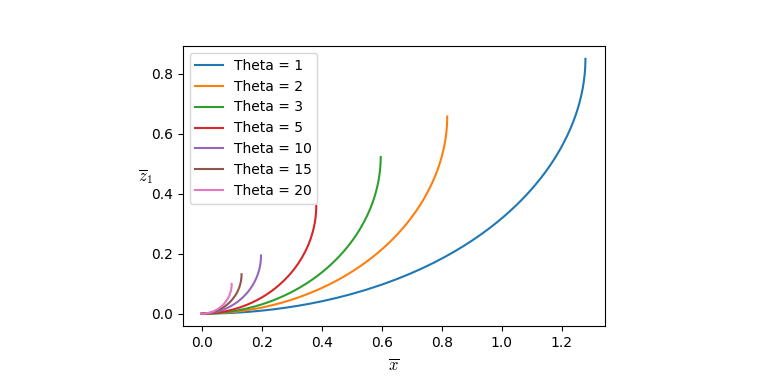
\includegraphics[width=0.85\linewidth]{WriteUp/images/bottom curve.png}
    \caption{Graphs of $\tilde{f}_1$ which solves equation \ref{less than} for $\theta=1,2,3,5,10,15,20$ where $\theta = 4/\bar{R}_0 - 2\bar{h}$ is the constant difference between the radius of curvature of the cap,$\bar{R}_0$, (section B) and the depth of the bubble, $\bar{h}$}
    \label{fig:5}
\end{figure}
As $\phi \rightarrow \pi/2$, $\frac{d\bar{z}_1}{dx} \rightarrow \infty$. This means our solver cannot compute the solution for $\phi> \pi/2$. What we do instead, is we can use the computed values for $\bar{z}_1$ and $\bar{x}$ at $\phi=\pi/2$ as initial conditions for equations \ref{greater than}. In a similar way to before, we can transform the equations \ref{greater than} into
\begin{align}
     \frac{d\bf{x}}{d\bar{z}_1}=\begin{bmatrix}
           \frac{v}{\sqrt{1-v^2}} \\
           -2\bar{z}_1 + \frac{\sqrt{1-v^2}}{\bar{x}}-\theta \\
         \end{bmatrix},
\end{align}
where $ \bf{x} = \begin{bmatrix}
    \bar{x}\\v
\end{bmatrix}$ and $v=\cos\phi$. We can then once again use $\texttt{solve\_ivp}$ to get a full solution to \ref{less than} and \ref{greater than}.let this solution be denoted by the function $F$ where
\begin{align}
    F(\bar{x},\theta,\phi)= \begin{cases}
        f_1(\bar{x},\theta) \;\;\;\;\; \text{for } \phi>\pi/2\\
        \tilde{f_1}(\bar{x},\theta) \;\;\;\;\; \text{for } \phi<\pi/2
    \end{cases}
\end{align}
In figure \ref{fig:6} we once again see a singularity form as $\phi \rightarrow \pi$. Although not exact, the gap between the $y$-axis and where the solutions ends gives an indication on what sort of shape the spherical cap should be. This is helpful later when we need to make an initial guess for another solver.
\begin{figure}
    \centering
    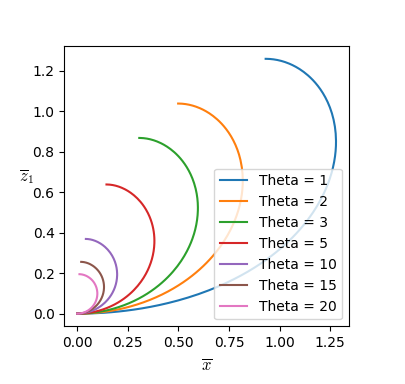
\includegraphics[width=0.65\linewidth]{WriteUp/images/top and bottom curve.png}
    \caption{Graphs of $F$ which solves equation \ref{less than} and \ref{greater than} for $\theta=1,2,3,5,10,15,20$ where $\theta = 4/\bar{R}_0 - 2\bar{h}$ is the constant difference between the radius of curvature of the cap,$\bar{R}_0$, (section B) and the depth of the bubble, $\bar{h}$.}
    \label{fig:6}
\end{figure}

\subsection{Solving for Segment (C)}

The equations generating segment (C) are very similar to segment (A), unfortunately, the boundary conditions make it much harder to solve. Segment (C) is the meniscus of the bubble and we would like it to flatten out at infinity. This means we have the boundary conditions $\phi \rightarrow 0$, $\bar{z} \rightarrow 0$ as $x \rightarrow \infty$. These conditions are unable to be implemented numerically, instead we can consider initial conditions close to zero, i.e. $\bar{z}=\phi=0.00001$ at $\bar{x}=\bar{x}_0$. We can then denote $\bar{z}=f_2(\bar{x},\bar{x}_0)$ as a solution to \ref{C_transformed}.

We once again see singularities forming in figure \ref{fig:7}. For the $\theta$ values for which we calculated solutions for segment A earlier, we want to consider $\bar{x}_0$ between around 4 and 8. We see from the figure that larger values of $\bar{x}_0$ are undefined in the domain of the solution to segment A. This allows us to narrow the search for the correct $\bar{x}_0$ to match with a given $\theta$.
\begin{figure}
    \centering
    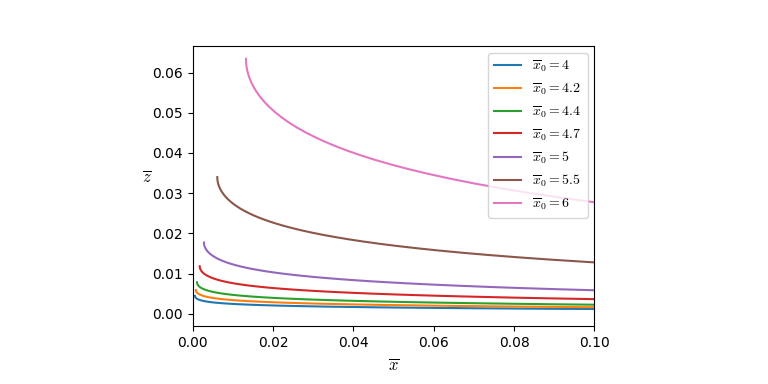
\includegraphics[width=0.85\linewidth]{WriteUp/images/menisc.png}
    \caption{Graphs of $f_2$ which solves equation \ref{C_transformed} for $\bar{x}_0=4,4.2,4.4,4.7,5,5.5,6$ where $\bar{x}_0$ is the initial $x$ coordinate we use for the Runge-Kutta method. These lines correspond to the meniscus formed due to the droplet resting above the surface level.}
    \label{fig:7}
\end{figure}

\subsection{Matching solutions for the Segments}

We are now able to calculate an explicit description of the interface for each individual section, but we still have many unknown variables we need to solve for. We want each section to meet at the same point and match derivatives at that point. applying these constraints we get the following system of equations:
\begin{align}
    \bar{z}&=F(\bar{x},\theta,\phi) - \bar{h} \\
    \bar{z}&=f_2(\bar{x},\bar{x}_0) \\
    \bar{z}&=\sqrt{\bar{R}_0^2-\bar{x}^2} - \bar{l}=f_3(\bar{x},\bar{R}_0)-\bar{l} \\
    \theta&=\frac{4}{\bar{R}}-2\bar{h}
\end{align}
and
\begin{align}
    \frac{d}{d\bar{x}}F(\bar{x},\theta,\phi)&=\frac{d}{d\bar{x}}f_2(\bar{x},\bar{x}_0) = \frac{d}{d\bar{x}}f_3(\bar{x},\bar{R}_0)
\end{align}
We can notice that $\frac{d}{d\bar{x}}f_3(\bar{x},\bar{R}_0)$ is always negative and that $\frac{d}{d\bar{x}}F(\bar{x},\theta,\phi)$ is only negative when $\phi>\pi/2$, i.e. when $F(\bar{x},\theta,\phi)=f_1(\bar{x},\theta)$. Using this we can reduce our system down to seven unknowns and six equations to solve, allowing us to have a free variable in $\theta$

We can further reduce this highly non-linear system to two variables. For a fixed $\theta$, we can consider this system in terms of $\bar{x}$ and $\bar{x}_0$ only. By fixing $\theta$ we can solve \ref{greater than} and \ref{less than} to obtain $f_1(\bar{x},\theta)$. We can then solve \ref{C_transformed} to obtain $f_2(\bar{x},\bar{x}_0)$. We can then obtain
\begin{align}
    \bar{h} = f_1(\bar{x},\theta) - f_2(\bar{x},\bar{x}_0),
\end{align}
and
\begin{align}
    \bar{R}_0=\frac{4}{2\bar{h} + \theta}.
\end{align}
Then we are able to calculate $f_3(\bar{x},\bar{R}_0)$ and finally
\begin{align}
    \bar{l} = f_3(\bar{x},\bar{R}_0)-f_1(\bar{x},\theta).
\end{align}
This reduces out problem to finding the roots of
\begin{align}\label{root 1}
    \frac{d}{d\bar{x}}f_1(\bar{x},\theta) -\frac{d}{d\bar{x}}f_2(\bar{x},\bar{x}_0) &=0 \\ \label{root 2}
    \frac{d}{d\bar{x}}f_1(\bar{x},\theta) - \frac{d}{d\bar{x}}f_3(\bar{x},\bar{R}_0) &=0
\end{align}
\subsection{Solutions}
We are now able to start computing solutions. In order to find the roots of \ref{root 1} and \ref{root 2}, we once again use SciPy. Due to the highly non-linear system we are solving, SciPy's root finding algorithms can be unreliable without a good initial guess. We are able to use data from \textit{TOBA} \cite{toba1959drop} as an initial guess for $\theta=2$, from there we could use our solution as an initial guess for $\theta=2.1$. This allows us to compute solutions for almost any $\theta$.

\begin{figure}
    \centering
    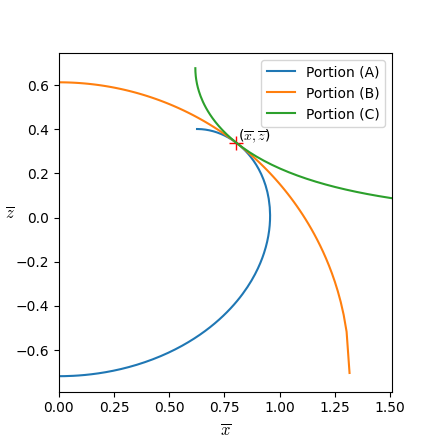
\includegraphics[width=0.85\linewidth]{WriteUp/images/combined theta=1.6.png}
    \caption{Solutions to full system for $\theta=1.6$. We can see each section meets at the point $(\bar{x},\bar{z})$ and that the derivatives match with one another}
    \label{fig:8}
\end{figure}

After computing a solution for a given $\theta$, we are able to calculate the bubble's nondimensional width. We note that $\theta$ is inversely proportional to this width as can be seen in figure \ref{fig:10}.
\begin{figure}
    \centering
    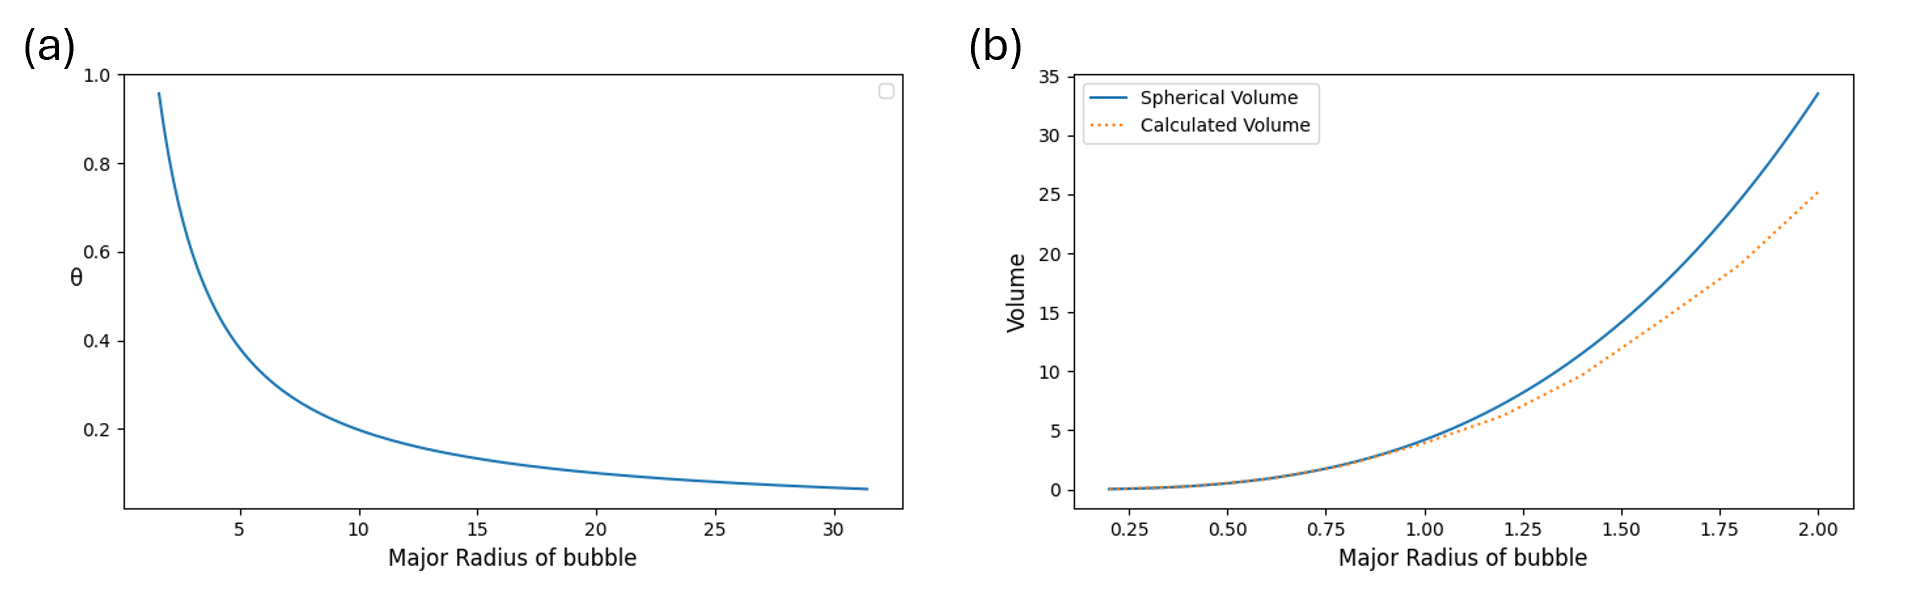
\includegraphics[width=0.85\linewidth]{WriteUp/images/Radius and volume.png}
    \caption{Figure (a) shows the size of the major radius (width) of the bubble for varying values of $\theta$, we can see an inversely proportional relationship between the major radius and $\theta$. Figure (b) shows the calculated volume of the bubble for a given radius. We see for smaller radii, the calculated volume is almost exactly that of a sphere.}
    \label{fig:10}
\end{figure}

For $\theta<1$ the solver becomes quite unreliable. This is due to the domain of $f_1$ shrinking, causing $f_1'$ to become incredibly sensitive to small changes in $\bar{x}$. This problem can be ignored however, as in this report we are considering bubbles formed at sea. As stated before, the scale of these bubbles is of order O($1$mm), transforming the radii we calculated for each theta (as shown in \ref{fig:8}) using the capillary constant for water ($a=2.71$ \cite{rapp2016microfluidics}) we find that for $\theta<0.9$ the radius of the bubble is greater than $5$mm. We can therefore safely ignore these small $\theta$ values as they do not correspond to any of the type of bubbles we are considering.
\begin{figure}
    \centering
    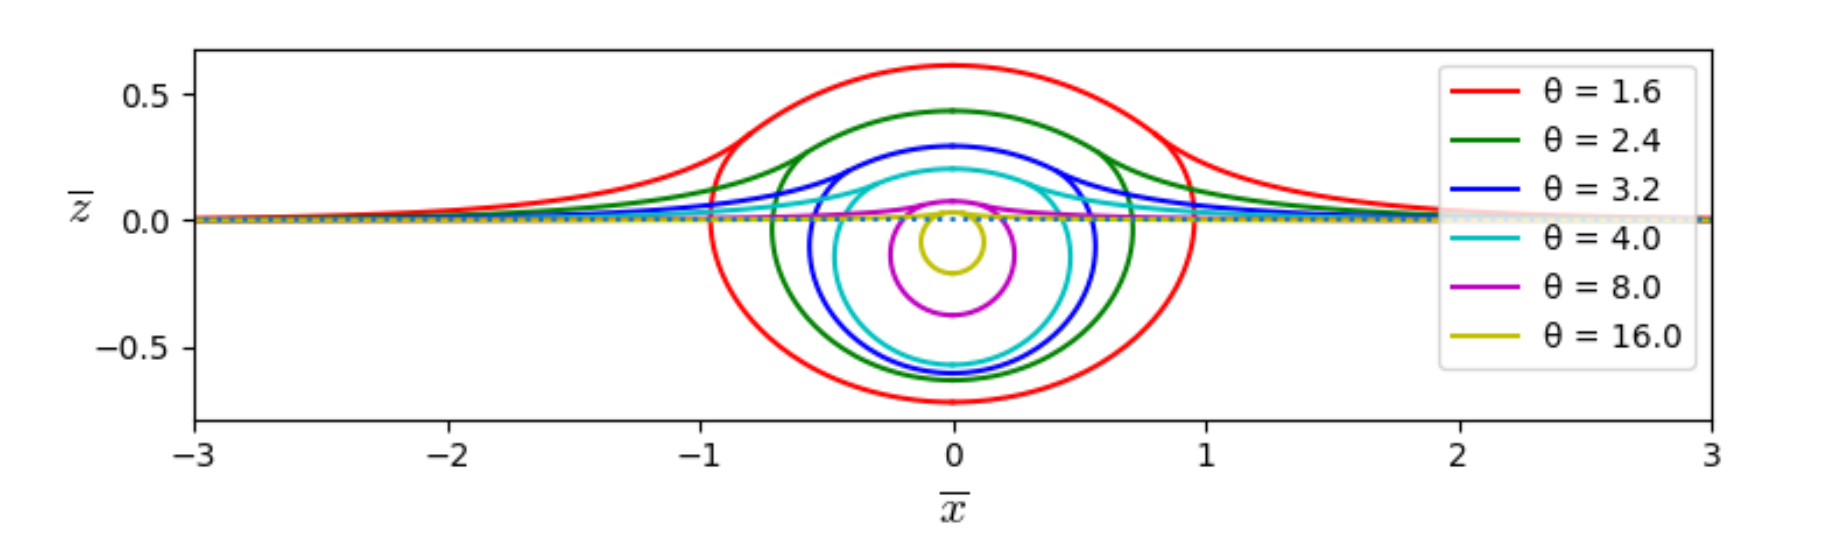
\includegraphics[width=0.85\linewidth]{WriteUp/images/many bubbles ontop one another.png}
    \caption{Solutions to full system for $\theta=1.6,2.4,3.2,4.0,8.0,16.0$}
    \label{fig:9}
\end{figure}
In figure \ref{fig:9} we see a clear trend in the shape of the bubble as $\theta$ increases. For larger values we see surface tension forces dominate, resulting in a spherical bubbles floating tangent to the surface of the water. As the bubble gets larger, the gravitational forces increase, causing the cap of the bubble to rise further above the water level. Figure \ref{fig:11} shows the shape of air bubbles in sea water for radii between $3.5$mm and $0.18$mm.

\begin{figure}
    \centering    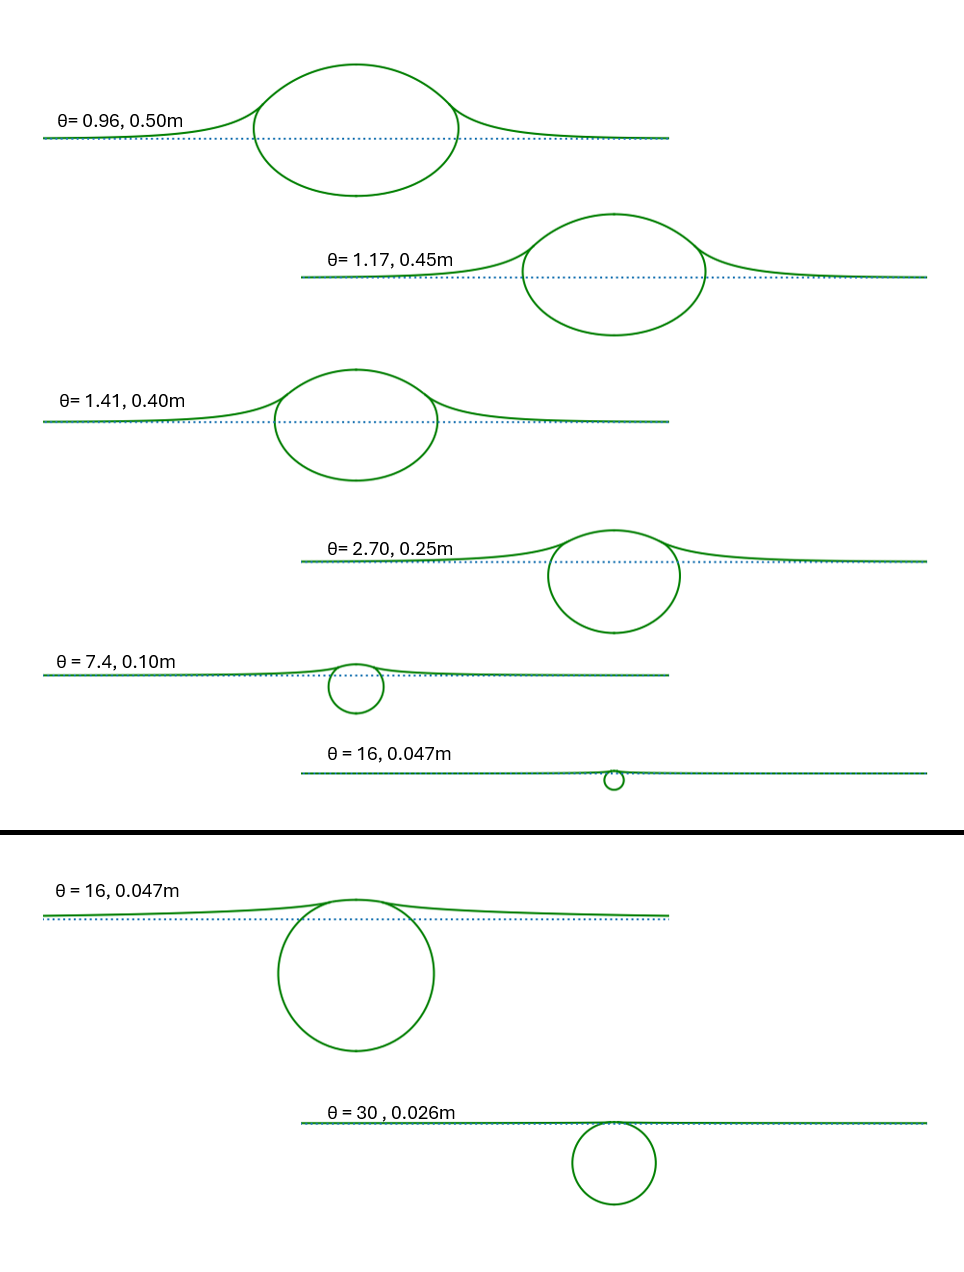
\includegraphics[width=0.95\linewidth]{WriteUp/images/Bubble profiles.png}
    \caption{Various bubble profiles scaled with $a=2.71mm$ corresponding to the capillary length of water under standard conditions \cite{rapp2016microfluidics}. The last two interfaces $\theta=16,30.8$ are scaled up. We see as $\theta$ decreases, the shape of the interface approaches the shape of a sphere just beneath the surface.}
    \label{fig:11}
\end{figure}
